\documentclass[a4paper]{llncs}

\usepackage[utf8]{inputenc}
\usepackage[T1]{fontenc}
\usepackage{amssymb}
\usepackage{graphicx}
\usepackage{url}
\usepackage{float}
\usepackage{booktabs}
\usepackage{tabularx}
\usepackage{enumitem}
\setlist[itemize]{noitemsep, topsep=3pt, parsep=0pt, partopsep=0pt}
\usepackage{pdflscape}

\renewcommand{\refname}{Bibliografia}

\raggedbottom

\setcounter{tocdepth}{3}

% Comando personalizado para a tabela de especificação (estilo Teórica T5, slide 39)
\newcommand{\ucspec}[7]{
\begin{table}[H]
    \centering
    \footnotesize
    \setlength{\tabcolsep}{4pt}
    \renewcommand{\arraystretch}{1.1}
    \begin{tabularx}{\textwidth}{|l|X|}
        \hline
        \textbf{Actor} & #1 \\ \hline
        \textbf{Use case name} & #2 \\ \hline
        \textbf{Description} & #3 \\ \hline
        \textbf{Precondition} & #4 \\ \hline
        \textbf{Postcondition} & #5 \\ \hline
        \textbf{Main flow} & #6 \\ \hline
        \textbf{Alternative path} & #7 \\ \hline
    \end{tabularx}
\end{table}
}

\begin{document}

\mainmatter

\title{Relatório Técnico - Iteração 02\\Sistema de Gestão de Supermercado}
\titlerunning{Relatório Técnico - Iteração 02}

\author{Grupo: 1DB\_3 \\
Tomás Bastos (1251506) \and Igor Almeida (1251054) \and \\
Guilherme Asevedo (1251002) \and Rui Silva (1251443)}
\institute{ISEP - Licenciatura em Engenharia de Telecomunicações e Informática}

\maketitle

\begin{abstract}
Este relatório documenta a fase de design e implementação do sistema de gestão de inventário e vendas para um supermercado, desenvolvido em C++17 com programação orientada a objetos. O documento apresenta a arquitetura em camadas (Model-View-Controller estendido com Services, Repository, DTOs e Mappers), diagramas de design das classes implementadas, e os casos de uso concretizados nesta iteração. A aplicação utiliza persistência em ficheiros CSV e interface de linha de comandos.
\\
\textbf{Palavras-chave:} C++, MVC, Design de Software, UML, Gestão de Supermercado, Arquitetura em Camadas, DTO, Singleton.
\end{abstract}

\section{Introdução}
O objetivo deste projeto é criar uma aplicação para gerir um supermercado, a aplicação vai ter um ADMIN, CAIXAs e CLIENTEs.

O ADMIN é responsável por gerir o catálogo da loja, incluindo criar, editar, listar e remover PRODUTOs. Tem também a habilidade de gerir CATEGORIAs de PRODUTOs, configurar PROMOÇÕEs temporárias com percentagens de desconto e intervalos de datas, e repor níveis de stock a PRODUTOs que já existem. Adicionalmente, o ADMIN irá gerir contas de CAIXA (criando-as e removendo-as), gerir a base de dados de CLIENTEs (registando, editando, listando e removendo CLIENTEs), e consultar estatísticas de desempenho globais e por CAIXA, como a faturação e o volume de VENDAs.

O CAIXA pode iniciar e processar VENDAs, adicionando PRODUTOs e quantidades, aplicando descontos automáticos de PROMOÇÕEs ativas e concluindo transações com diferentes métodos de pagamento. Pode também associar um CLIENTE a uma VENDA em curso através do seu NIF, consultar o quantidade de PONTOS atual de um CLIENTE e visualizar o seu próprio histórico de desempenho e total faturado. Após concluir uma VENDA, o sistema irá gerar um RECIBO com os detalhes dos PRODUTOs, totais e método de pagamento utilizado.

Os CLIENTEs registados no sistema acumularão PONTOS de fidelização com base nas suas compras (ex: 1 ponto por cada 10\texteuro{} gastos). Estes PONTOS poderão ser utilizados para descontos em compras futuras. O sistema armazenará os dados do CLIENTE, incluindo o seu NIF, nome e quantidade de PONTOS de fidelização associado.

Este relatório inclui histórias de utilizador, requisitos funcionais e não funcionais (utilizando o modelo FURPS+), o modelo de domínio, especificações e diagramas de casos de uso, e o design de software baseado no padrão Model-View-Controller (MVC). A aplicação será desenvolvida em C++17 utilizando programação orientada a objetos, com persistência de dados através de ficheiros CSV externos.

\section{Análise de Requisitos}

\subsection{User Stories}

\subsubsection{Administrador (ADMIN)}
\begin{itemize}
    \item \textbf{US01:} Como ADMIN, eu quero criar novos PRODUTOS para poder atualizar o catálogo do supermercado.
    \item \textbf{US02:} Como ADMIN, eu quero apagar PRODUTOS do sistema para que os PRODUTOS que já não existam deixem de estar na base de dados.
    \item \textbf{US03:} Como ADMIN, eu quero listar todos os PRODUTOS existentes para que possa consultar o inventário.
    \item \textbf{US04:} Como ADMIN, eu quero aceder a estatísticas globais dos CAIXAS para avaliar o desempenho do supermercado.
    \item \textbf{US05:} Como ADMIN, eu quero adicionar e remover CAIXAs (adição/remoção) para controlar quem tem acesso ao sistema de VENDAS.
    \item \textbf{US06:} Como ADMIN, eu quero comprar stock para PRODUTOS existentes para garantir que não falta PRODUTOS.
    \item \textbf{US07:} Como ADMIN, eu quero gerir o registo de CLIENTES (criar/editar/apagar) para manter a base de dados de CLIENTES atualizada.
    \item \textbf{US08:} Como ADMIN, eu quero criar e gerir PROMOÇÕES (percentagem, data início, data fim) para incentivar as VENDAS.
    \item \textbf{US09:} Como ADMIN, eu quero gerir CATEGORIAS de produtos para organizar o inventário e aplicar impostos diferentemente para cada CATEGORIA.
\end{itemize}

\subsubsection{CAIXA}
\begin{itemize}
    \item \textbf{US10:} Como CAIXA, eu quero listar PRODUTOS e consultar preços para informar os CLIENTES.
    \item \textbf{US11:} Como CAIXA, eu quero realizar VENDAS (registando PRODUTOS e quantidades) para processar as compras dos CLIENTES.
    \item \textbf{US12:} Como CAIXA, eu quero concluir VENDAS com diferentes métodos de pagamento e emitir RECIBOS para documentar a transação.
    \item \textbf{US13:} Como CAIXA, eu quero consultar o meu histórico e informação individual para saber o meu desempenho.
    \item \textbf{US14:} Como CAIXA, eu quero associar uma VENDA a um CLIENTE (via NIF) para que este possa acumular PONTOS.
    \item \textbf{US15:} Como CAIXA, eu quero consultar o quantidade de PONTOS de um CLIENTE para informar o CLIENTE sobre os PONTOS que ele tem.
    \item \textbf{US16:} Como CAIXA, eu quero que o sistema aplique automaticamente os descontos ativos no momento da VENDA sem intervenção manual.
    \item \textbf{US17:} Como CAIXA, eu quero consultar o detalhe de RECIBOS de vendas passadas para esclarecer dúvidas dos clientes.
\end{itemize}

\subsection{Requisitos Funcionais (RF)}
\begin{itemize}
    \item \textbf{RF01:} O sistema deve permitir a criação de um novo PRODUTO (nome, preço\_base), criando um \texttt{id} único automaticamente.
    \item \textbf{RF02:} O sistema deve permitir a remoção de um PRODUTO pelo seu \texttt{id}.
    \item \textbf{RF03:} O sistema deve listar todos os PRODUTOS com os seus respetivos detalhes e stock existente.
    \item \textbf{RF04:} O sistema deve permitir o registo e remoção de utilizadores com perfil de CAIXA.
    \item \textbf{RF05:} O sistema deve calcular estatísticas de performance (faturação e volume) por CAIXA e globalmente.
    \item \textbf{RF06:} O sistema deve gerir o ciclo de vida de uma VENDA (iniciar, adicionar itens, cancelar, concluir).
    \item \textbf{RF07:} O sistema deve validar a disponibilidade de stock durante o registo de itens na VENDA.
    \item \textbf{RF08:} O sistema deve registar o método de pagamento e mostrar um RECIBO após a conclusão da venda.
    \item \textbf{RF09:} O sistema deve identificar o utilizador e restringir acesso a funcionalidades baseadas em ser um ADMIN ou um CAIXA.
    \item \textbf{RF10:} O sistema deve garantir a persistência de dados em ficheiros externos.
    \item \textbf{RF11:} O sistema deve permitir a gestão de CLIENTES (NIF, Nome) e garantir que o NIF é único.
    \item \textbf{RF12:} O sistema deve permitir associar um CLIENTE a uma VENDA em curso.
    \item \textbf{RF13:} O sistema deve calcular e atribuir PONTOS ao CLIENTE após uma venda concluída (ex: 1 PONTO por cada 10€).
    \item \textbf{RF14:} O sistema deve aplicar automaticamente o resgate de PONTOS para descontos no valor total da VENDA, caso o CLIENTE possua saldo suficiente.
    \item \textbf{RF15:} O sistema deve permitir a criação de PROMOÇÕES com intervalo de datas (início e fim) e percentagem de desconto.
    \item \textbf{RF16:} O sistema deve validar se uma PROMOÇÃO está ativa (data atual dentro do intervalo) antes de aplicar o desconto.
    \item \textbf{RF17:} O sistema deve permitir associar uma PROMOÇÃO a um PRODUTO ou a uma CATEGORIA de produtos.
    \item \textbf{RF18:} O sistema deve garantir que, no caso de existir mais de uma promoções aplicáveis, apenas a que desconte mais dinheiro para o cliente é aplicada.
\end{itemize}

\subsection{Requisitos Não Funcionais (FURPS+)}

\subsubsection{Functionality (F)}
\begin{itemize}
    \item \textbf{RNF01 (Persistência de Dados):} O sistema deve garantir que o armazenamento de dados será em ficheiros CSV locais.
\end{itemize}
\subsubsection{Usability (U)}
\begin{itemize}
    \item \textbf{RNF02 (Estrutura de Menus):} O sistema deve permitir uma navegação por menus na CLI, por seleção numérica (0-9).
\end{itemize}
\subsubsection{Reliability (R)}
\begin{itemize}
    \item \textbf{RNF03 (Recuperação de Erro):} O sistema deve verificar os tipos de dados de entrada (ex: carateres em campos numéricos) e pedir uma nova introdução caso o tipo de dado esteja errado, sem perder o estado da transação ativa.
    \item \textbf{RNF04 (Integridade de Dados):} O sistema deve garantir que todas as transações que forem concluídas devem ser registadas num ficheiro.
\end{itemize}
\subsubsection{Performance (P)}
O sistema deve responder prontamente às interações do utilizador na CLI.

\subsubsection{Supportability (S)}
\begin{itemize}
    \item \textbf{RNF06 (Portabilidade/Build):} O projeto deve ser compilável através de CMake (versão 3.10 ou superior) em ambiente Linux (GCC/Clang) e Windows (MSVC).
\end{itemize}
\subsubsection{+ (Restrições de Implementação)}
\begin{itemize}
    \item \textbf{RNF07 (Norma da Linguagem):} O código fonte deve ser compatível com a norma C++17 (ISO/IEC 14882:2017).
\end{itemize}

\section{Modelação de Domínio}

\begin{figure}[H]
    \centering
    \makebox[\textwidth][c]{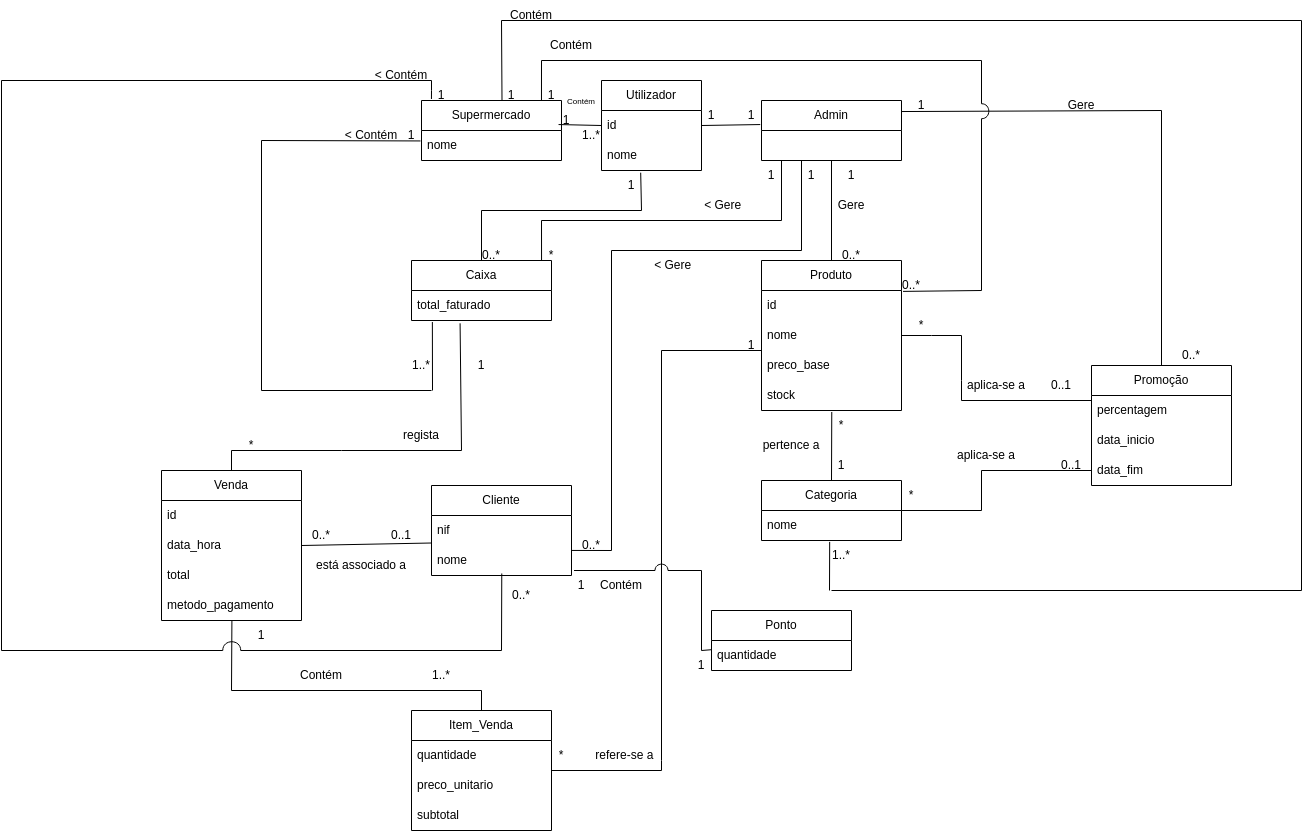
\includegraphics[width=1.4\textwidth]{diagramas/DomainModel/domain_model(2).drawio.png}}
    \caption{Diagrama UML de Domínio}
    \label{fig:domain_model}
\end{figure}

\section{Design de Software}

\begin{figure}[H]
    \centering
    \makebox[\textwidth][c]{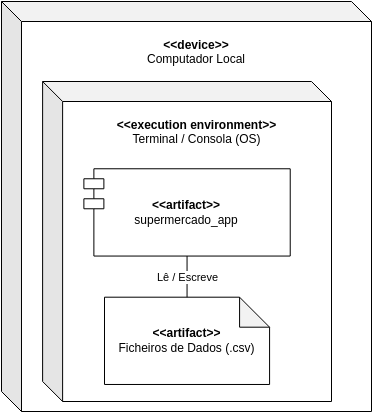
\includegraphics[width=1.2\textwidth]{diagramas/design/physical_architecture.drawio.png}}
    \caption{Diagrama de Arquitetura Física}
    \label{fig:physical_architecture}
\end{figure}

\begin{figure}[H]
    \centering
    \makebox[\textwidth][c]{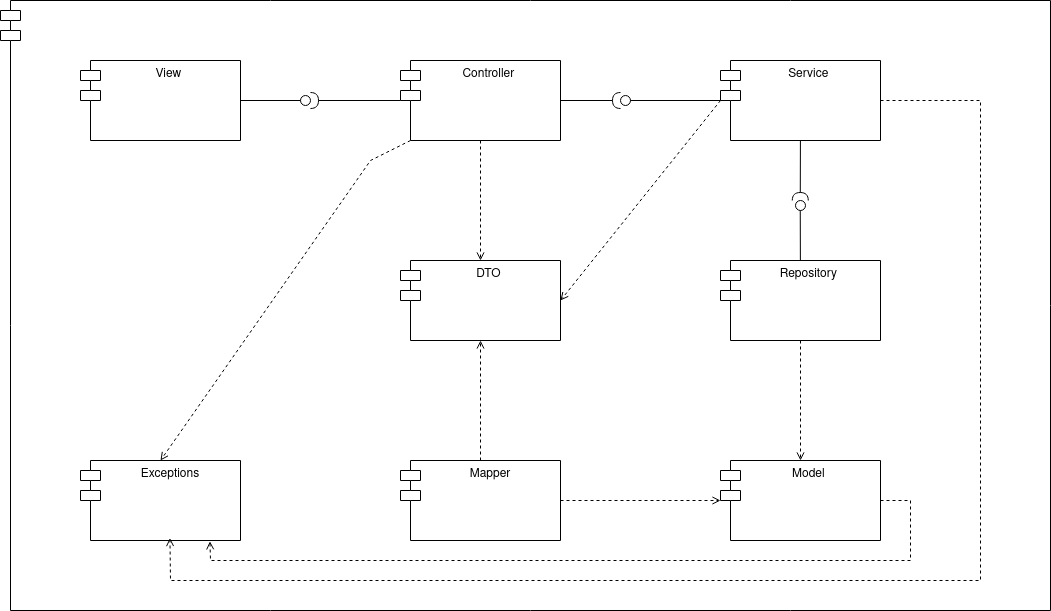
\includegraphics[width=1.2\textwidth]{diagramas/design/logical_architecture.drawio.png}}
    \caption{Diagrama de Arquitetura Lógica}
    \label{fig:logical_architecture}
\end{figure}

\begin{figure}[H]
    \centering
    \makebox[\textwidth][c]{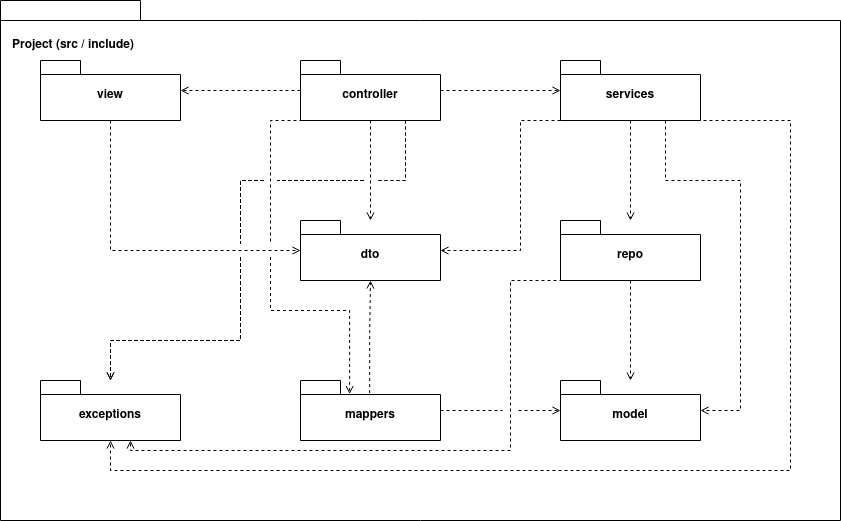
\includegraphics[width=1.2\textwidth]{diagramas/design/code_organization.drawio.png}}
    \caption{Organização do Código}
    \label{fig:code_organization}
\end{figure}

\begin{figure}[H]
    \centering
    \makebox[\textwidth][c]{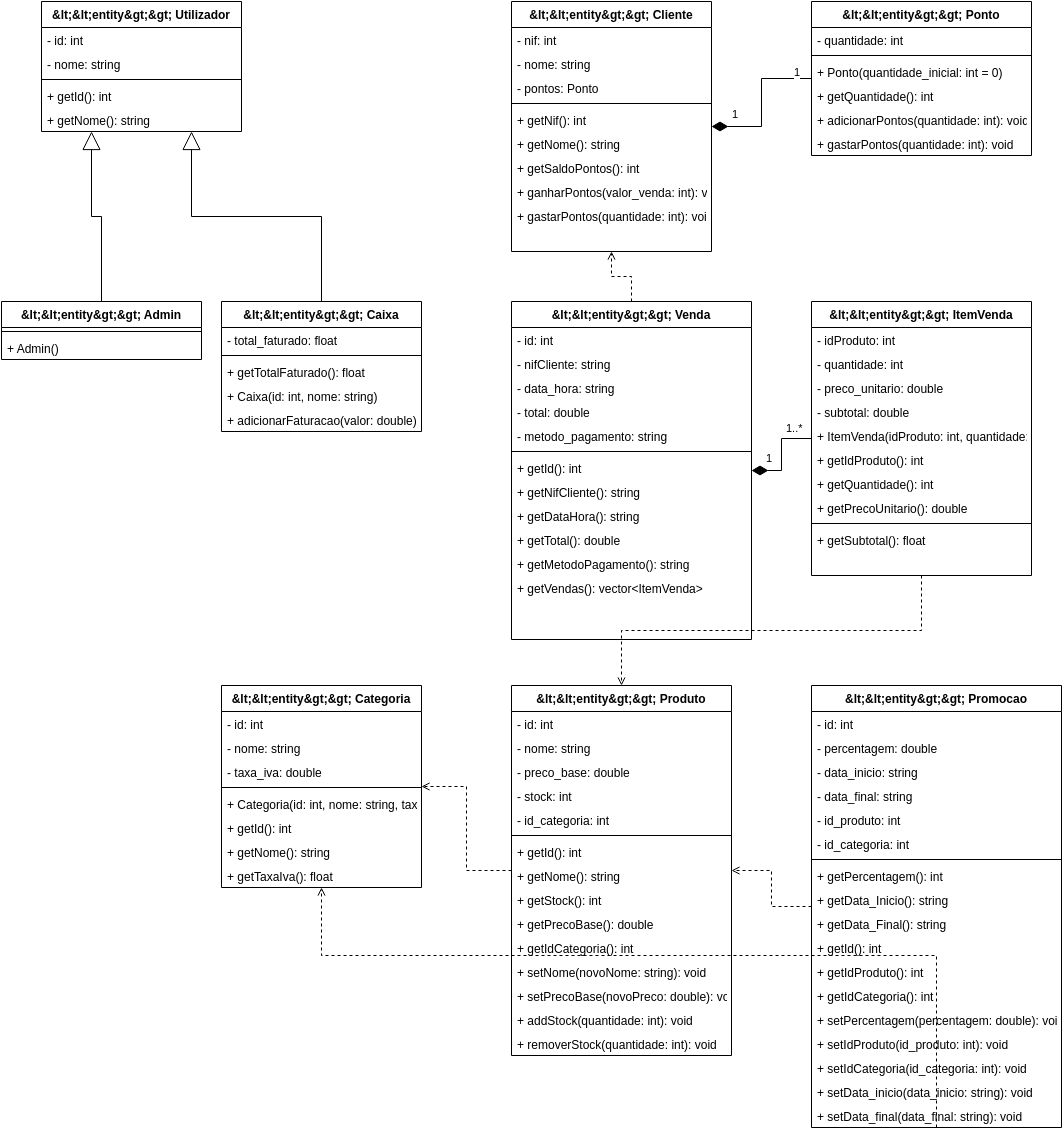
\includegraphics[width=1.2\textwidth]{diagramas/design/model_class_diagram.drawio.png}}
    \caption{Diagrama de Classes do Modelo (Design Class Diagram)}
    \label{fig:model_class_diagram}
\end{figure}

\begin{figure}[H]
    \centering
    \makebox[\textwidth][c]{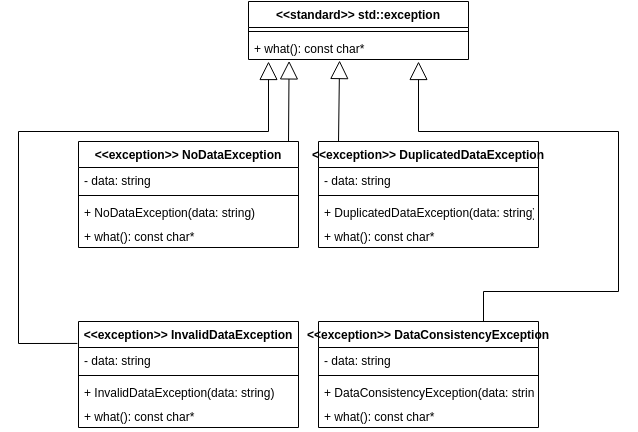
\includegraphics[width=1.0\textwidth]{diagramas/design/exceptions_class_diagram.drawio.png}}
    \caption{Diagrama de Classes das Exceções}
    \label{fig:exceptions_class_diagram}
\end{figure}

\begin{figure}[H]
    \centering
    \makebox[\textwidth][c]{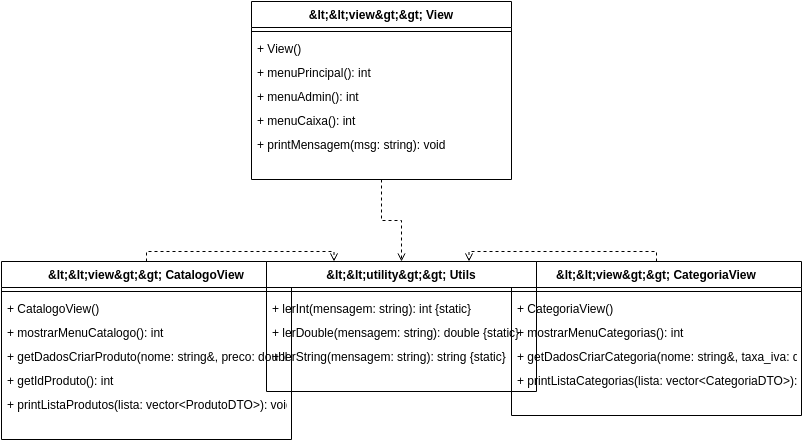
\includegraphics[width=1.1\textwidth]{diagramas/design/views_class_diagram.drawio.png}}
    \caption{Diagrama de Classes das Views}
    \label{fig:views_class_diagram}
\end{figure}

\begin{figure}[H]
    \centering
    \makebox[\textwidth][c]{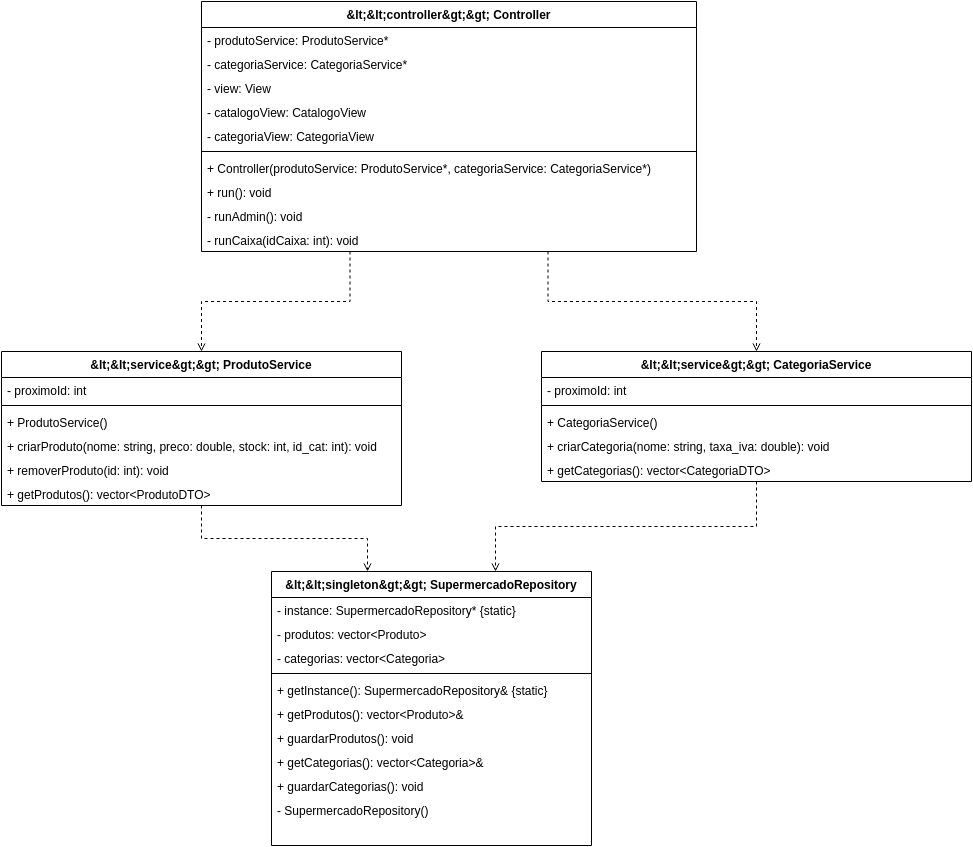
\includegraphics[width=1.0\textwidth]{diagramas/design/controllers_services_class_diagram.drawio.png}}
    \caption{Diagrama de Classes do Controller, Services e Repository}
    \label{fig:controllers_services_class_diagram}
\end{figure}

\begin{figure}[H]
    \centering
    \makebox[\textwidth][c]{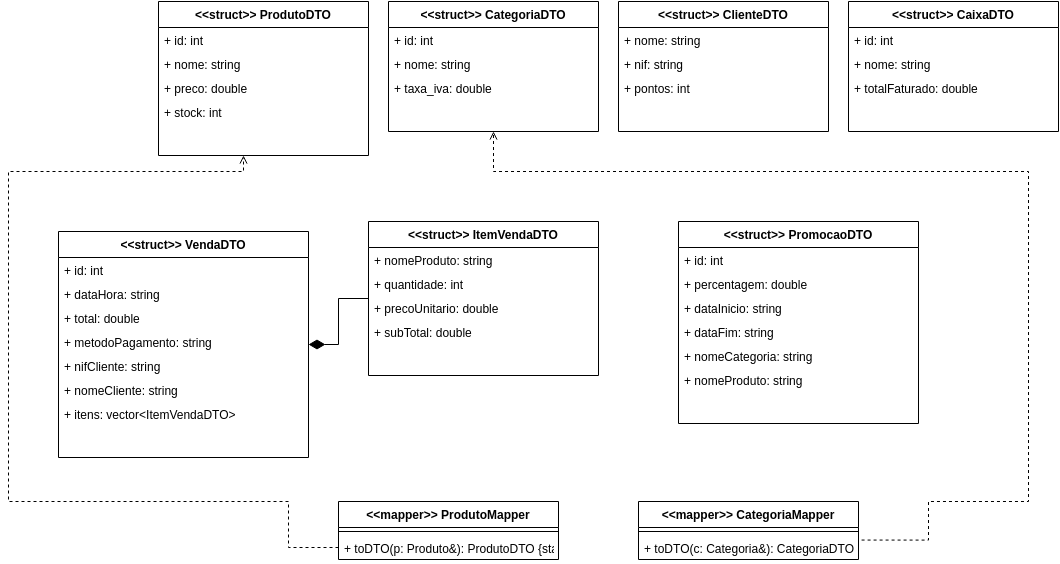
\includegraphics[width=1.1\textwidth]{diagramas/design/dtos_mappers_class_diagram.drawio.png}}
    \caption{Diagrama de DTOs e Mappers}
    \label{fig:dtos_mappers_class_diagram}
\end{figure}

\subsection{Padrão Model-View-Controller (MVC)}

O sistema foi dividido em camadas seguindo o padrão Model-View-Controller que foi estendido com Services, Repository, DTOs e Mappers:

\begin{enumerate}
    \item \textbf{Model:} Contém as classes de dados (\texttt{Produto}, \texttt{Categoria}, \texttt{Cliente}, \texttt{Venda}, \texttt{ItemVenda}, \texttt{Promocao}, \texttt{Ponto}, \texttt{Caixa}, \texttt{Admin}, \texttt{Utilizador}). Estas classes \texttt{<<entity>>}, representam as entidades do domínio e não conhecem a parte do View.
    \item \textbf{View:} Responsável por toda a interação com o utilizador seja a enviar dados ou a pedir dados. Inclui as classes \texttt{View}, \texttt{CatalogoView}, \texttt{CategoriaView} e \texttt{Utils} (validar o input do utilizador).
    \item \textbf{Controller:} A classe \texttt{Controller} é a classe que orquestra o funcionamento do sistema. Recebe os Services no construtor, gere a navegação dos menus e deixa todas as operações de negócio aos Services. Trata exceções com blocos \texttt{try/catch} e comunica resultados através da View.
    \item \textbf{Service:} As classes \texttt{ProdutoService} e \texttt{CategoriaService}  contêm a lógica de negócio e validações. Geram IDs automáticos e coordenam a persistência através do Repository.
    \item \textbf{Repository:} A classe \texttt{SupermercadoRepository}  centraliza toda a persistência de dados em ficheiros CSV. É acedida via \texttt{getInstance()} e expõe referências para os vectores internos.
    \item \textbf{DTO:} Estruturas de transferência de dados: \texttt{ProdutoDTO}, \texttt{CategoriaDTO}, \texttt{ClienteDTO}, \texttt{CaixaDTO}, \texttt{VendaDTO}, \texttt{ItemVendaDTO}, \texttt{PromocaoDTO} que transportam dados entre camadas sem expor os Models diretamente às Views.
    \item \textbf{Mappers:} Classes \texttt{ProdutoMapper} e \texttt{CategoriaMapper} com métodos estáticos \texttt{toDTO()} que convertem Modelos em DTOs.
    \item \textbf{Exceptions:} Quatro classes de exceção \texttt{NoDataException}, \texttt{DuplicatedDataException}, \texttt{InvalidDataException}, \texttt{DataConsistencyException} que herdam de \texttt{std::exception} e são usadas pelos Services e capturadas pelo Controller.
\end{enumerate}

O fluxo de uma operação típica é: \textbf{View} recolhe o input, \textbf{Controller} chama \textbf{Service}, \textbf{Service} valida e usa \textbf{Repository}, \textbf{Mapper} converte Model, DTO, \textbf{Controller} passa DTO à \textbf{View} para apresentar.

\subsection{Arquitetura de Ficheiros}

\begin{itemize}
    \item \textbf{\texttt{include/model/}} — Headers das entidades de domínio (\texttt{Produto.h}, \texttt{Categoria.h}, \texttt{Cliente.h}, \texttt{Venda.h}, etc.)
    \item \textbf{\texttt{include/view/}} — Headers das classes de interface (\texttt{View.h}, \texttt{CatalogoView.h}, \texttt{CategoriaView.h}, \texttt{Utils.h})
    \item \textbf{\texttt{include/controller/}} — Header do orquestrador (\texttt{Controller.h})
    \item \textbf{\texttt{include/services/}} — Headers da lógica de negócio (\texttt{ProdutoService.h}, \texttt{CategoriaService.h})
    \item \textbf{\texttt{include/repo/}} — Header do repositório Singleton (\texttt{SupermercadoRepository.h})
    \item \textbf{\texttt{include/dto/}} — Estruturas de transferência de dados (\texttt{ProdutoDTO.h}, \texttt{CategoriaDTO.h}, etc.)
    \item \textbf{\texttt{include/mappers/}} — Conversores Model-DTO (\texttt{ProdutoMapper.h}, \texttt{CategoriaMapper.h})
    \item \textbf{\texttt{include/exceptions/}} — Classes de exceção (\texttt{NoDataException.h}, etc.)
    \item \textbf{\texttt{src/}} — Implementações correspondentes a cada header, espelhando a mesma estrutura de pastas.
\end{itemize}

A compilação é gerida pelo \texttt{CMakeLists.txt} (C++17, CMake 3.10+) e o ponto onde o programa começa é o \texttt{main.cpp}.

\subsection{Padrões de Desenho Aplicados (GRASP)}
Exemplos de classes onde usamos certos Padroes de desenho:

\begin{itemize}
    \item \textbf{Creator:} O padrão \textit{Creator} é aplicado na classe \texttt{SupermercadoRepository}. No método \texttt{carregarProdutos()} ocorre a instanciação dos objetos \texttt{Produto} depois da a leitura do ficheiro CSV e extração da informaçao la dentro, sendo o repositório o agregador que contém e gere as instâncias de produtos.
    \item \textbf{Controller:} O padrão \textit{Controller} é implementado através da classe \texttt{Controller}, que atua como o orquestrador do sistema. Esta classe recebe os eventos da interface (View) e dá ordens de execução para as outras camadas.
    \item \textbf{Service:} O padrão \textit{Service} é utilizado na classe \texttt{ProdutoService}, onde está a lógica de negócio associada aos produtos (como a atribuição de um ID automático e as verificações de que os dados são válidos).
\end{itemize}

\subsection{Interface de Utilizador}

\begin{figure}[H]
    \centering
    \makebox[\textwidth][c]{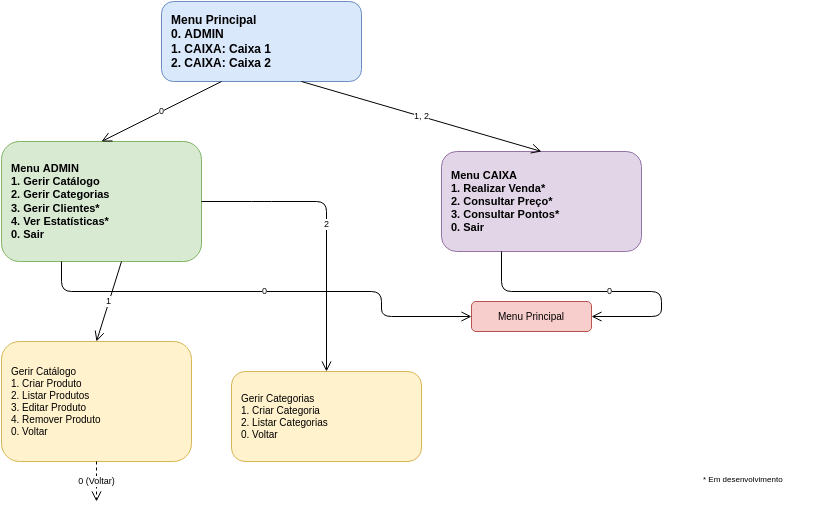
\includegraphics[width=1.1\textwidth]{diagramas/design/ui_navigation.drawio.png}}
    \caption{Árvore de Navegação da Interface de Utilizador}
    \label{fig:ui_navigation}
\end{figure}

\section{Modelo de Casos de Uso}
Nesta secção detalhamos as interações entre os atores e o sistema.

\begin{figure}[H]
    \centering
    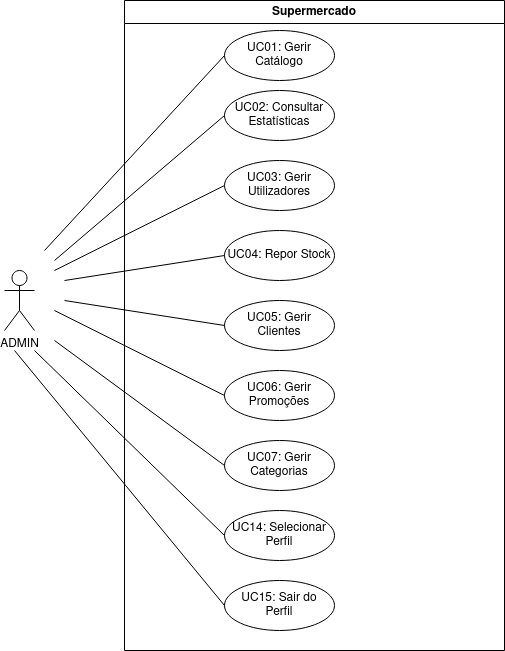
\includegraphics[width=0.8\textwidth]{diagramas/UseCaseDiagrams/use_case_diagram_admin.png}
    \caption{Diagrama de Casos de Uso - Administrador}
    \label{fig:uc_admin}
\end{figure}

\begin{figure}[H]
    \centering
    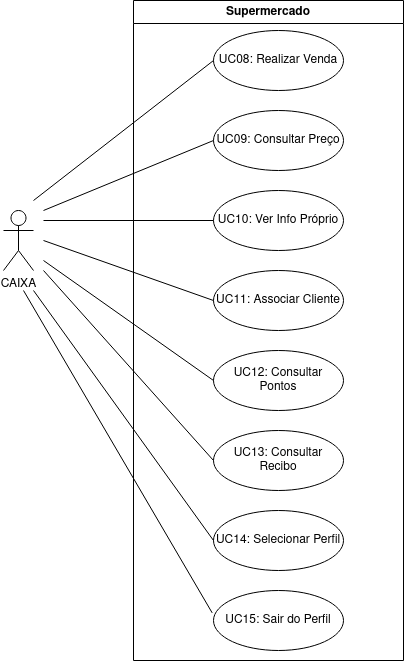
\includegraphics[width=0.8\textwidth]{diagramas/UseCaseDiagrams/use_case_diagram_caixa.png}
    \caption{Diagrama de Casos de Uso - Caixa}
    \label{fig:uc_caixa}
\end{figure}

\begin{table}[H]
    \centering
    \footnotesize
    \setlength{\tabcolsep}{4pt}
    \begin{tabularx}{\textwidth}{lllX}
        \toprule
        \textbf{ID} & \textbf{Caso de Uso} & \textbf{Ator(es)} & \textbf{Descrição Resumida} \\ \midrule
        UC01 & Gerir Catálogo & ADMIN & Permite criar, editar, listar e remover PRODUTOS. \\
        UC02 & Consultar Estatísticas & ADMIN & Gera relatórios de faturação e volume por CAIXA ou global. \\
        UC03 & Gerir Utilizadores & ADMIN & Permite o registo e remoção de contas de perfil 'CAIXA'. \\
        UC04 & Repor Stock & ADMIN & Incrementa a quantidade disponível de um PRODUTO existente. \\
        UC05 & Gerir CLIENTES & ADMIN & Permite o registo, edição e remoção de perfis de CLIENTE. \\
        UC06 & Gerir PROMOÇÕES & ADMIN & Permite criar, editar e apagar PROMOÇÕES temporárias. \\
        UC07 & Gerir CATEGORIAS & ADMIN & Agrupar PRODUTOS para fins de IVA e Descontos. \\
        UC08 & Realizar VENDA & CAIXA & Inicia transação, adiciona itens, calcula total e regista pagamento. \\
        UC09 & Consultar Preço & CAIXA & Pesquisa e exibe o preço unitário de um PRODUTO pelo seu ID. \\
        UC10 & Ver Info Própria & CAIXA & Exibe dados do funcionário e total de vendas faturado. \\
        UC11 & Associar CLIENTE & CAIXA & Durante a VENDA, permite ligar a transação a um CLIENTE. \\
        UC12 & Consultar Pontos & CAIXA & Visualizar quantidade de PONTOS do CLIENTE. \\
        UC13 & Consultar RECIBO & CAIXA & Consultar e visualizar o RECIBO de uma VENDA terminada. \\
        UC14 & Selecionar Perfil & ADMIN, CAIXA & Identifica o utilizador e o seu papel para aceder ao sistema. \\
        UC15 & Sair do Perfil & ADMIN, CAIXA & Termina a sessão do utilizador atual. \\ \bottomrule
    \end{tabularx}
    \caption{Lista de Casos de Uso}
    \label{tab:use_cases}
\end{table}

\subsection{Especificações de Casos de Uso}

\subsubsection{UC01: Gerir Catálogo}
\ucspec{ADMIN}{Gerir Catálogo}{Permite criar, editar, listar e remover PRODUTOS.}{ADMIN selecionado no sistema.}{Catálogo de PRODUTOS atualizado na base de dados.}{
1. O ADMIN seleciona a opção "gestão do catálogo". \newline
2. O sistema mostra as opções disponíveis (Criar, Editar, Listar, Remover). \newline
3. O ADMIN seleciona "Criar". \newline
4. O sistema pede os dados (nome, preço base, stock inicial, categoria). \newline
5. O ADMIN introduz os dados. \newline
6. O sistema valida os dados, cria um ID automático e grava. \newline
7. O sistema confirma o sucesso da operação.
}{
\textbf{3.a. Listar:} \newline
1. O ADMIN seleciona "Listar". \newline
2. O sistema apresenta a lista de todos os produtos e respetivos detalhes. \newline
3. O UC termina. \newline
\textbf{3.b. Editar:} \newline
1. O ADMIN seleciona a opção "Editar". \newline
2. O sistema pede o ID do produto. \newline
3. O ADMIN escreve o ID. \newline
4. O sistema mostra os dados atuais e pede novos dados. \newline
5. O ADMIN insere os novos dados. \newline
6. O sistema valida e atualiza o produto. \newline
7. O UC termina. \newline
\textbf{3.c. Remover:} \newline
1. O ADMIN seleciona "Remover". \newline
2. O sistema pede o ID do produto. \newline
3. O ADMIN insere o ID. \newline
4. O sistema confirmação. \newline
5. O ADMIN confirma. \newline
6. O sistema remove o produto \newline
7. O UC termina.
}
\subsubsection{UC02: Consultar Estatísticas}
\ucspec{ADMIN}{Consultar Estatísticas}{Permite visualizar relatórios de faturação global ou por CAIXA.}{ADMIN selecionado no sistema.}{N/A}{
1. O ADMIN seleciona a opção de "consulta de estatísticas". \newline
2. O sistema pede o filtro (global ou por utilizador CAIXA). \newline
3. O ADMIN escolhe o filtro. \newline
4. O sistema cria e apresenta o relatório de faturação e quantidade de vendas.
}{N/A}
\subsubsection{UC03: Gerir Utilizadores}
\ucspec{ADMIN}{Gerir Utilizadores}{Permite registar e remover contas de perfil 'CAIXA'.}{ADMIN selecionado no sistema.}{Lista de CAIXAs é atualizada.}{
1. O ADMIN seleciona a opção "gestão de utilizadores". \newline
2. O sistema mostra as opções (Registar, Listar, Remover). \newline
3. O ADMIN seleciona "Registar". \newline
4. O ADMIN introduz os dados do novo CAIXA (nome). \newline
5. O sistema verifica os dados e cria a conta de perfil 'CAIXA'. \newline
6. O sistema confirma a criação com sucesso.
}{
\textbf{3.b. Remover:} \newline
1. O ADMIN seleciona a opção "Remover". \newline
2. O sistema pede o ID do CAIXA. \newline
3. O ADMIN escrve o ID. \newline
4. O sistema pede confirmação. \newline
5. O ADMIN confirma. \newline
6. O sistema remove a conta e informa o sucesso. \newline
7. O UC termina.
}
\subsubsection{UC04: Repor Stock}
\ucspec{ADMIN}{Repor Stock}{Aumenta a quantidade disponível de um PRODUTO existente.}{ADMIN selecionado no sistema.}{Stock do PRODUTO é incrementado.}{
1. O ADMIN pesquisa o PRODUTO pelo ID. \newline
2. O sistema mostra os dados atuais do PRODUTO. \newline
3. O ADMIN introduz a quantidade a adicionar ao stock. \newline
4. O sistema atualiza o valor do stock na base de dados. \newline
5. O sistema confirma o novo valor total de stock.
}{N/A}
\subsubsection{UC05: Gerir CLIENTES}
\ucspec{ADMIN}{Gerir CLIENTES}{Permite registar, editar e remover perfis de CLIENTE.}{ADMIN selecionado no sistema.}{Base de dados de CLIENTES atualizada.}{
1. O ADMIN escolhe a opção "gestão de CLIENTES". \newline
2. O sistema mostra as opções (Registar, Editar, Listar, Remover). \newline
3. O ADMIN seleciona a opção "Registar". \newline
4. O ADMIN introduz o NIF e o nome do CLIENTE. \newline
5. O sistema valida o NIF, coloca o quantidade de PONTOS a zero e guarda o perfil. \newline
6. O sistema confirma o sucesso da operação.
}{
\textbf{3.a. Listar:} \newline
1. O ADMIN seleciona a opção "Listar". \newline
2. O sistema apresenta a lista de todos os CLIENTES (NIF, Nome, quantidade de PONTOS). \newline
3. O UC termina. \newline
\textbf{3.b. Editar:} \newline
1. O ADMIN seleciona a opção "Editar". \newline
2. O sistema solicita o NIF do CLIENTE. \newline
3. O ADMIN insere o NIF. \newline
4. O sistema mostra os dados atuais e solicita novo nome. \newline
5. O ADMIN insere o novo nome. \newline
6. O sistema atualiza o perfil. \newline
7. O UC termina. \newline
\textbf{3.c. Remover:} \newline
1. O ADMIN seleciona a opção "Remover". \newline
2. O sistema solicita o NIF do CLIENTE. \newline
3. O ADMIN insere o NIF. \newline
4. O sistema pede confirmação. \newline
5. O ADMIN confirma. \newline
6. O sistema remove o perfil e informa o sucesso. \newline
7. O UC termina.
}

\subsubsection{UC06: Gerir PROMOÇÕES}
\ucspec{ADMIN}{Gerir PROMOÇÕES}{Permite criar e configurar regras de descontos temporários.}{ADMIN selecionado no sistema.}{Base de dados de PROMOÇÕES atualizada.}{
1. O ADMIN escolhe a opção "Gestão de PROMOÇÕES". \newline
2. O sistema mostra as opções (Criar, Listar, Remover). \newline
3. O ADMIN seleciona "Criar". \newline
4. O ADMIN define a percentagem de desconto e as datas de inicio e final. \newline
5. O ADMIN associa a PROMOÇÃO a um PRODUTO ou CATEGORIA específica. \newline
6. O sistema valida e guarda a regra de desconto. \newline
7. O sistema confirma o sucesso.
}{
\textbf{3.a. Listar:} \newline
1. O ADMIN seleciona "Listar". \newline
2. O sistema apresenta a lista de todas as PROMOÇÕES ativas e agendadas. \newline
3. O UC termina. \newline
\textbf{3.b. Remover:} \newline
1. O ADMIN seleciona a opção "Remover". \newline
2. O sistema solicita a identificação da promoção. \newline
3. O ADMIN seleciona a promoção a remover. \newline
4. O sistema pede confirmação. \newline
5. O ADMIN confirma. \newline
6. O sistema remove a regra de desconto e informa o sucesso. \newline
7. O UC termina.
}

\subsubsection{UC07: Gerir CATEGORIAS}
\ucspec{ADMIN}{Gerir CATEGORIAS}{Permite agrupar PRODUTOS em CATEGORIAS para find de impostos e descontos.}{ADMIN selecionado no sistema.}{Lista de CATEGORIAS atualizada.}{
1. O ADMIN escolhe a opção "gestão de categorias". \newline
2. O sistema apresenta as opções (Criar, Listar, Remover). \newline
3. O ADMIN seleciona "Criar". \newline
4. O ADMIN introduz o nome da nova CATEGORIA e a taxa de IVA dessa CATEGORIA. \newline
5. O sistema valida os dados e cria a CATEGORIA. \newline
6. O sistema confirma a criação com sucesso.
}{
\textbf{3.a. Listar:} \newline
1. O ADMIN seleciona "Listar". \newline
2. O sistema apresenta a lista de todas as categorias. \newline
3. O UC termina. \newline
\textbf{3.b. Remover:} \newline
1. O ADMIN seleciona a opção "Remover". \newline
2. O sistema solicita o ID da categoria. \newline
3. O ADMIN insere o ID. \newline
4. O sistema remove a categoria e informa o sucesso. \newline
5. O UC termina.
}

\subsubsection{UC08: Realizar VENDA}
\ucspec{CAIXA}{Realizar VENDA}{Realiza uma VENDA de PRODUTOS a um CLIENTE ou a alguém que não é um CLIENTE.}{CAIXA selecionado no sistema.}{VENDA registada, o stock atualizado e RECIBO emitido.}{
1. O CAIXA seleciona a opção de iniciar uma nova VENDA. \newline
2. O CAIXA introduz o ID e quantidade de cada PRODUTO. \newline
3. O sistema valida o item, calcula o subtotal e apresenta-o. \newline
4. O CAIXA termina a introdução de itens. \newline
5. O sistema calcula o total final (aplica impostos e promoções). \newline
6. O CAIXA regista o pagamento. \newline
7. O sistema acaba a VENDA e emite o RECIBO.
}{
\textbf{6.a. Cancelar VENDA:} \newline
1. O CAIXA solicita o cancelamento da venda antes do pagamento. \newline
2. O sistema pede confirmação. \newline
3. O CAIXA confirma. \newline
4. O sistema descarta os dados da venda em curso e liberta o stock reservado. \newline
5. O UC termina.
}

\subsubsection{UC09: Consultar Preço}
\ucspec{CAIXA}{Consultar Preço}{Pesquisa e mostra o preço de um PRODUTO pelo seu ID.}{CAIXA selecionado no sistema.}{N/A (Consulta).}{
1. O CAIXA escreve o ID do PRODUTO. \newline
2. O sistema pesquisa o ID. \newline
3. O sistema apresenta o nome e o preço do PRODUTO.
}{N/A}

\subsubsection{UC10: Ver Info Própria}
\ucspec{CAIXA}{Ver Info Própria}{Mostra os dados do utilizador CAIXA e o total de dinheiro das vendas acumulado.}{CAIXA selecionado no sistema.}{N/A (Consulta).}{
1. O CAIXA solicita a opção de ver a sua informação. \newline
2. O sistema apresenta os dados do perfil (ID, nome) e o total faturado acumulado.
}{N/A}

\subsubsection{UC11: Associar CLIENTE}
\ucspec{CAIXA}{Associar CLIENTE}{Durante uma VENDA, associa o CLIENTE à transação.}{VENDA em curso.}{CLIENTE está associado à VENDA.}{
1. O CAIXA solicita a opção de "associação de um CLIENTE." \newline
2. O CAIXA introduz o NIF do CLIENTE. \newline
3. O sistema valida o NIF e mostra o nome correspondente. \newline
4. O sistema liga o CLIENTE à VENDA atual.
}{N/A}

\subsubsection{UC12: Consultar Pontos}
\ucspec{CAIXA}{Consultar Pontos}{Permite consultar o quantidade de PONTOS atual de um CLIENTE.}{CAIXA selecionado no sistema.}{N/A (Consulta).}{
1. O CAIXA introduz o NIF do CLIENTE. \newline
2. O sistema pesquisa o perfil correspondente. \newline
3. O sistema apresenta o quantidade de PONTOS atual do CLIENTE.
}{N/A}

\subsubsection{UC13: Consultar RECIBO}
\ucspec{CAIXA}{Consultar RECIBO}{Permite visualizar uma venda já feita.}{CAIXA selecionado no sistema.}{N/A (Consulta).}{
1. O CAIXA seleciona uma das vendas que efetuou. \newline
2. O sistema pesquisa os dados da venda. \newline
3. O sistema cria e mostra o RECIBO detalhado no ecrã.
}{N/A}

\subsubsection{UC14: Selecionar Perfil}
\ucspec{ADMIN, CAIXA}{Selecionar Perfil}{Permite ao utilizador do programa identificar-se (ADMIN ou CAIXA) e aceder ao menu de opções correspondente.}{Sistema no menu de seleção inicial.}{Utilizador selecionado e menu de funções ativo.}{
1. O utilizador seleciona o seu perfil (ADMIN ou um CAIXA específico) de uma lista apresentada. \newline
2. O sistema verifica as permissões do perfil. \newline
3. O sistema apresenta o menu de operações ao papel selecionado.
}{N/A}

\subsubsection{UC15: Sair do Perfil}
\ucspec{ADMIN, CAIXA}{Sair do Perfil}{Termina a sessão do utilizador atual.}{Utilizador com ADMIN selecionado OU CAIXA selecionado no sistema.}{Sessão terminada e sistema regressa ao menu de seleção inicial.}{
1. O utilizador seleciona a opção de "Logout". \newline
2. O sistema limpa os dados de sessão atuais. \newline
3. O sistema regressa ao menu de seleção de perfil inicial.
}{N/A}

\subsection{Casos de Uso Implementados}

Dos 15 casos de uso identificados na iteração anterior, 4 foram implementados nesta iteração: UC01 (Gerir Catálogo), UC07 (Gerir Categorias), UC14 (Selecionar Perfil) e UC15 (Sair do Perfil). Os restantes vão ser implementados na próxima iteração.

\begin{figure}[H]
    \centering
    
\includegraphics[width=0.7\textwidth]{diagramas/SSDs/uc01.png}
    \caption{UC01: Gerir Catálogo (Cenário de Criação)}
\end{figure}

\begin{figure}[H]
    \centering
    
\includegraphics[width=0.7\textwidth]{diagramas/SSDs/uc07.png}
    \caption{UC07: Gerir CATEGORIAS}
\end{figure}

\begin{figure}[H]
    \centering
    
\includegraphics[width=0.7\textwidth]{diagramas/SSDs/uc14.png}
    \caption{UC14: Selecionar Perfil}
\end{figure}

\begin{figure}[H]
    \centering
    
\includegraphics[width=0.7\textwidth]{diagramas/SSDs/uc15.png}
    \caption{UC15: Sair do Perfil}
\end{figure}

\subsection{Restantes Casos de Uso}

Os restantes casos de uso, já foram documentados com especificações e diagramas de sequência, mas ainda não foram implementados.

\begin{figure}[H]
    \centering
    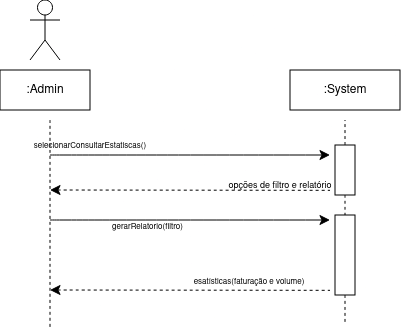
\includegraphics[width=0.7\textwidth]{diagramas/SSDs/uc02.png}
    \caption{UC02: Consultar Estatísticas}
\end{figure}

\begin{figure}[H]
    \centering
    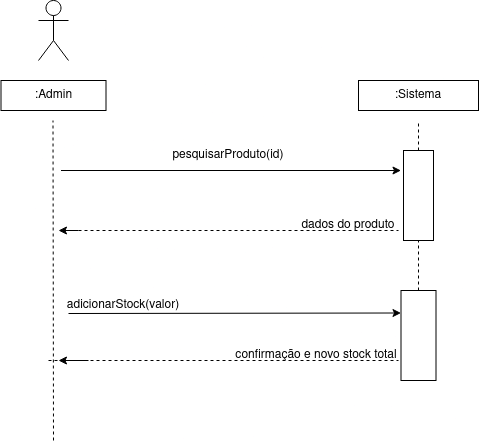
\includegraphics[width=0.7\textwidth]{diagramas/SSDs/uc04.png}
    \caption{UC04: Repor Stock}
\end{figure}

\begin{figure}[H]
    \centering
    
\includegraphics[width=0.7\textwidth]{diagramas/SSDs/uc05.png}
    \caption{UC05: Gerir CLIENTES (Cenário de Registo)}
\end{figure}

\begin{figure}[H]
    \centering
    
\includegraphics[width=0.7\textwidth]{diagramas/SSDs/uc06.png}
    \caption{UC06: Gerir PROMOÇÕES (Cenário de Criação)}
\end{figure}

\begin{figure}[H]
    \centering
    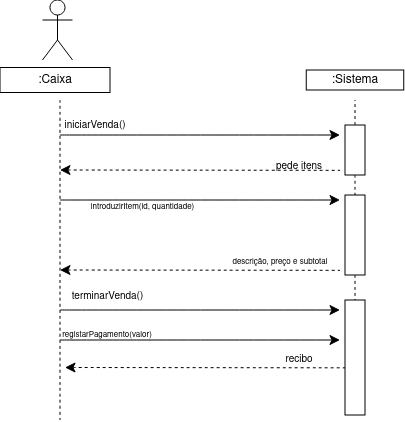
\includegraphics[width=0.7\textwidth]{diagramas/SSDs/uc08.png}
    \caption{UC08: Realizar VENDA}
\end{figure}

\begin{figure}[H]
    \centering
    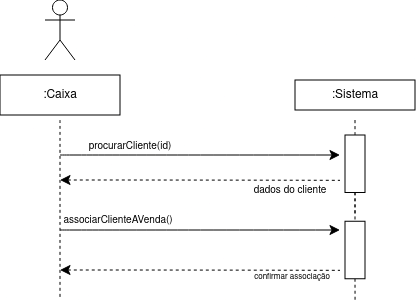
\includegraphics[width=0.7\textwidth]{diagramas/SSDs/uc11.png}
    \caption{UC11: Associar CLIENTE}
\end{figure}

\begin{figure}[H]
    \centering
    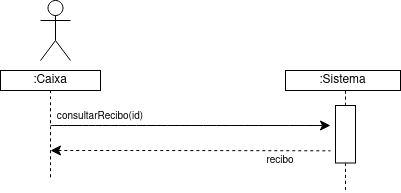
\includegraphics[width=0.7\textwidth]{diagramas/SSDs/uc13.png}
    \caption{UC13: Consultar RECIBO}
\end{figure}

\section{Glossário}
\begin{description}
    \item[ADMIN] Tipo de UTILIZADOR com o papel de gestão e controlo total das operações do sistema.
    \item[CAIXA] Tipo de UTILIZADOR que atua como funcionário operador do sistema de vendas.
    \item[CATEGORIA] Agrupamento de produtos com características semelhantes (ex: Bebidas, Talho, Peixaria).
    \item[CLIENTE] Pessoa que compra PRODUTOS no supermercado, e que está registada no sistema para fidelização.
    \item[ESTATÍSTICA] Relatório de desempenho de faturação e volume de vendas por período ou operador.
    \item[MÉTODO DE PAGAMENTO] Forma como o cliente liquida o valor de uma venda (ex: Numerário, Cartão).
    \item[PONTO] Unidade de medida de fidelização que ao ser acumulada por compras é possível converter para ter descontos.
    \item[PRODUTO] Artigo com ID único, descrição, preço e stock.
    \item[PROMOÇÃO] Desconto percentual aplicado a produtos ou categorias num certo intervalo de tempo.
    \item[RECIBO] Comprovativo de uma venda concluída entregue ao cliente, que inclui o valor total pago, o método de pagamento e a lista de produtos comprados.
    \item[UTILIZADOR] Entidade base do sistema que agrupa atributos comuns de identificação, da qual derivam os perfis específicos de operação.
    \item[VENDA] Transação que associa produtos e um método de pagamento.
\end{description}

\section{Conclusão}
A segunda iteração foi dedicada ao design e à implementação do sistema. Usamos o padrão MVC estendido em mais camadas(Services, Exceptions, repo etc), o que nos permitiu organizar o código de forma clara e com responsabilidades bem definidas. No total, resultaram desta fase 10 classes de domínio (Model), 4 classes de interface (View), 2 Services, 1 Repository com padrão Singleton, 7 DTOs, 2 Mappers e 4 classes de exceção. Todo este design foi documentado através de 8 diagramas UML, um por cada aspeto relevante da arquitetura.
Do ponto de vista da implementação, conseguimos concluir 4 dos 15 casos de uso identificados na iteração anterior: Gerir Catálogo (UC01), Gerir Categorias (UC07), Selecionar Perfil (UC14) e Sair do Perfil (UC15). Aproveitámos também para rever os diagramas de sequência, tornando-os mais detalhados e de acordo com o fluxo real do sistema, mostrando a informação que percorre as camadas, da View até ao Repository, passando pelo Controller e pelo Service.
Para a próxima iteração, o objetivo é implementar os casos de uso que ainda faltam, com especial foco na gestão de Vendas, Clientes e Promoções. E realizar os testes unitários, utilizando o framework Google Test. 

\begin{thebibliography}{2}

\bibitem{fsoft_material}
ISEP: Fundamentos de Desenvolvimento de Software (FSOFT) - Material de Apoio (Aulas Teóricas e Guia do Projeto) (2025/2026)

\bibitem{cpp17}
ISO/IEC: ISO/IEC 14882:2017 - Programming languages -- C++. \url{https://www.iso.org/standard/68564.html} (2017)

\end{thebibliography}

\end{document}
